%-------------------------------------------------------------------------------
% yum_padsynth
%-------------------------------------------------------------------------------
%
% \file        yum_padsynth.tex
% \library     Documents
% \author      Chris Ahlstrom
% \date        2015-06-07
% \update      2022-05-09
% \version     $Revision$
% \license     $XPC_GPL_LICENSE$
%
%     Provides the PADsynth section of yoshimi-user-manual.tex.
%
%-------------------------------------------------------------------------------

\section{PADsynth}
\label{sec:padsynth}

   The \textsl{Yoshimi} PADsynth dialog is a complex dialog for creating a
   pad instrument,  "PADsynth" or "PADnote" is an engine that makes very
   beautiful pads and other instruments. (These instruments can be exported
   for use with other programs too).

   The PadSynth engine was designed by Paul Nasca and to the best of our
   knowledge there is no comparable type generally available. It starts with a
   waveform that is virtually identical to the one used by AddSynth. However,
   each harmonic of this waveform is then widened and shifted and blurred, by
   rendering it with a harmonic profile (frequency distribution). The resulting
   sound is similar to granular synthesis, but can be generated very
   efficiently from a set of perfectly looping wavetables. These wavetables
   need to be precomputed after a change, so none of the harmonic profile
   controls are real-time. Also, it is the wavetables that are called for
   actual sound generation after passing through the usual envelope controls
   (and this part of sound generation does work real-time).

   The PADsynth dialog consists of two major tabs,
   \textbf{Harmonic Structure} and \textbf{EnvelopesLFOs}.
   Each of these tabs is complex, so the discussion
   will break the tabs down by sub-sections.

   There is extra protection for a really huge PadSynth engine
   (that can potentially take tens of seconds to complete).
   For that time, any attempt to alter the part that contains the one
   that's updating will not accept any other changes,
   and will give the warning: \texttt{Part \textsl{n} busy}.

\subsection{PADsynth / Algorithm}
\label{subsec:padsynth_algorithm}

   The complexity of the PADsynth dailog reflects the complexity of the
   PADsynth algorithms themselves.

\subsubsection{PADsynth / Algorithm / General}
\label{subsubsec:padsynth_algorithm_general}

   The PADsynth algorithm generates very beautiful sounds, even if its idea is
   much simpler than other algorithms. It generates a perfectly looped
   wave-table sample which can be used in instruments. It easily generates
   sounds of ensembles, choirs, metallic sounds (bells) and many other types of
   sound.  Paul Nasca wanted to make this algorithm known, and everyone is
   welcome to learn and use this algorithm in one's projects or products
   (non-commercial or commercial).

   Quote \cite{zyndoc}:

   \begin{quotation}
      You will not be disappointed by this algorithm.

      I hope that this algorithm will be implemented in many software/hardware
      synthesizers. Use it, spread it, write about it, create beautiful
      instruments with it. If your synthesizer uses plenty of samples, you can
      use this algorithm to generate many ready-to-use samples.

      This algorithm, this page, the images, the implementations from this
      page, the audio examples, the parameter files from this page
      are released under Public Domain by Nasca Octavian Paul.
      e-mail: zynaddsubfx AT yahoo DOT com
   \end{quotation}

   In order to understand how this algorithm works, one needs to be familiar
   with how to think about musical instruments. Please read an introduction
   for the description of the meaning and the importance of bandwidth of each
   harmonic and randomness.

   This algorithm generates some large wave-tables that can be played at
   different speeds to get the desired sound. This algorithm describes only
   how these wave-tables are generated. The result is a perfectly looped
   wave-table.  Unlike other synthesis methods, which use the
   Inverse Fast Fourier Transform, this one does not use overlap/add methods
   and there is only one IFFT for the whole sample.

   The basic steps are:

   \begin{enumber}
      \item Make a very large array that represents the amplitude spectrum of
         the sound (all default values are zero).
      \item Generate the distribution of each harmonic in the frequency
         spectrum and add it to the array.
      \item Put random phases to each frequency of the spectrum.
      \item Do a single Inverse Fourier Transform of the whole spectrum. There
         is no need of any overlapping windows, because there is only one
         single IFFT for the whole sample.
   \end{enumber}

   The output is a sample which can be used as a wave-table.

%  In the next image, the steps are represented graphically:
%     TODO:  A GRAPHIC

\subsubsection{PADsynth / Algorithm / Harmonic Bandwidth}
\label{subsubsec:padsynth_algorithm_harmonic_bandwidth}

   We consider one harmonic (overtone) as being composed of many frequencies.
   These sine components of one harmonic are spread over a certain band of
   frequencies.  Higher harmonics have a wider bandwidth. In natural
   choirs/ensembles the bandwidth is proportional to the frequency of the
   harmonic.

%  Here is an example of a spectrum of an instrument generated by ZynAddSubFX:
%
%     TODO:  A GRAPHIC, full spectrum, closeup of the spectrum

%   The harmonics become wider and wider, until a certain frequency, where
%   they may merge into a noise band (as in the full spectrum image from above
%   shows). This is a normal thing and we recommend to not avoid this by
%   limiting the bandwidth of the harmonics.

   The harmonics become wider and wider, until a certain frequency, where
   they may merge into a noise band. This is quite normal and we recommend not
   suppressing this by limiting the bandwidth of the harmonics.

%  The frequency distribution of one harmonic/overtone (or the harmonic
%  profile).

   This describes the function of the spread of the harmonic.
   Here are some examples of how they can be spread:

   \begin{enumber}
      \item  A special case is where there is only a single sine component
         inside the harmonic In this case, the harmonic and the "sine
         component" are the same thing.
      \item  Detuned. In this case there are two sine components which are
         detuned.
      \item  Evenly spread inside the harmonic (all components have the same
         amplitude)
      \item  Normal (Gaussian) distribution. The sine components amplitude are
         bell-shaped. The largest amplitude is in the center of the band. This
         distribution gives the most natural sounds (it simulates a very, very
         large ensemble).
   \end{enumber}

   Of course, one can use many other profiles of the harmonic.
   \textsl{ZynAddSubFX}'s PADsynth module offers many ways to generate the
   harmonic profile.  Also, it's very important that the harmonic must have the
   same amplitude, regardless of the profile functions/parameters and the
   bandwidth.
   For many more details of this algorithm, see Paul Nasca's document
   \cite{zyndoc}.

\paragraph{Tip: Using the PADsynth}
\label{tips_using_the_padsynth}
\index{tips!padsynth usage}

   Keep in mind that the resulting wave-tables are perfectly looped.
   There are some sound-generation ideas to keep in mind:

   \begin{enumber}
      \item When using the wave-tables for instruments, on each Note On, start
         from a random position and not from the start. This avoids hearing the
         same sound on each keystroke.
      \item One can use the same wave-table for generating stereo sounds, by
         playing the same wave-table at different positions for left and right.
         The best method is to create a difference between left and
         right of N/2.
      \item Generate different wave-tables for different pitches and use the
         one that is closest to the desired pitch.
      \item Upsample or downsample the amplitude array of the harmonic before
         running the algorithm, according to the fundamental frequency. In this
         case we need to set a parameter "base\_frequency" which represents the
         frequency where the array is left unchanged.
   \end{enumber}

   Example:
   We have A\_orig[]={1,2,1,3,0,0,1,0} and base\_frequency is equal to 440 Hz
   Here are some cases:

   A[] for 440 Hz: is the same as A\_orig[]

   A[] for 220 Hz: is the A\_orig[] upsampled by factor of 2

   so: A[]={1, 1, 1.5, 2, 1.5, 1, 2, 3, 1.5, 0, 0, 0, 0.5, 1, 0.5, 0}

   (the original A\_orig amplitudes are shown as bold)

   A[] for 880 Hz: the A\_orig[] is downsampled by a factor of 2

   so: A[]={1.5, 2, 0, 0.5}

   A[] for F Hz: the A\_orig[] is scaled by a factor of 440/F.

   Even if this idea is very simple, the resulting sounds are very natural,
   because it keeps the spectrum constant according to the frequency of the
   harmonic and not to the number of the harmonics. This follows from the
   document where Paul Nasca describes some principles regarding synthesis.

\subsection{PADsynth / Harmonic Structure}
\label{subsec:padsynth_harmonic_structure}

\begin{figure}[H]
   \centering
   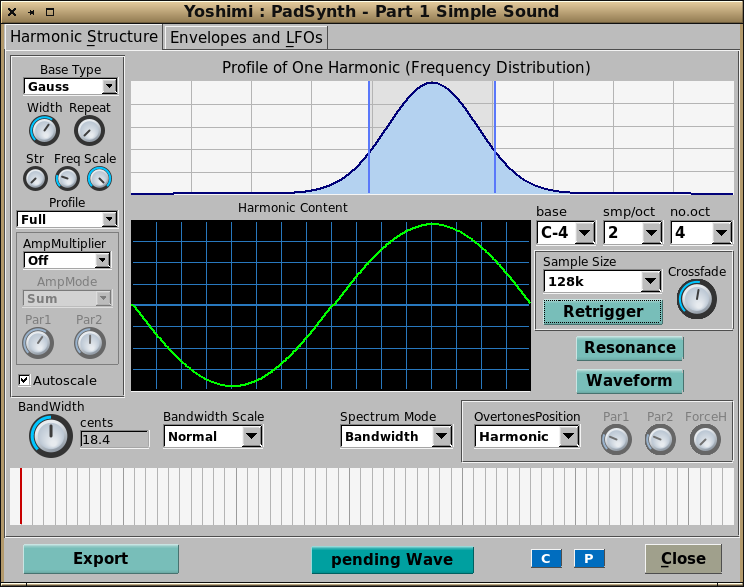
\includegraphics[scale=0.45]{2.2.0/padharmonic.png}
   \caption{PADsynth Edit Dialog}
   \label{fig:padsynth_edit_dialog}
\end{figure}

   Note how, in the newer versions of \textsl{Yoshimi}, the
   part number and part name are part of the window caption.
   There are a lot of parameter sections to keep track of, and to describe.

   \begin{enumber}
      \item \textbf{Basics} (section)
      \item \textbf{Harmonic} (section)
      \item \textbf{Resonance} (section)
      \item \textbf{Waveform} (section)
      \item \textbf{Bandwidth and Position} (section)
      \item \textbf{Export} (section)
      \item \textbf{C}
      \item \textbf{P}
      \item \textbf{Apply Changes}
      \item \textbf{Close}
   \end{enumber}

   Some of these elements have their own sections devoted to them, below.

\subsubsection{PADsynth / Harmonic Structure / Basics}
\label{subsubsec:padsynth_harmonic_structure_basics}

   \begin{enumber}
      \item \textbf{Base Type}
      \item \textbf{Width}
      \item \textbf{Repeat}
      \item \textbf{Str}
      \item \textbf{Freq}
      \item \textbf{Scale}
      \item \textbf{Full/Upper/Lower}
      \item \textbf{AmpMultiplier}
      \item \textbf{AmpMode}
      \item \textbf{Par1}
      \item \textbf{Par2}
   \end{enumber}

   \setcounter{ItemCounter}{0}      % Reset the ItemCounter for this list.

   \itempar{Base Type}{padsynth!harmonic type}
   Base Type of the Harmonic.
   This is the base shape used to widen and spread each harmonic:
   gauss, square, or double explonential.

\begin{figure}[H]
   \centering
   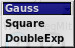
\includegraphics[scale=1.0]{bottom-panel/instrument-edit/PAD/base-type.jpg}
   \caption{Base Type of Harmonic}
   \label{fig:padsynth_base_type_of_harmonic}
\end{figure}

   Values: \texttt{Gauss*, Square, DoubleExp}

   \itempar{Width}{padsynth!harmonic width}
   Width of harmonic, the spread of a single peak within the profile.
   The lowest value yields a very thin
   \textbf{Profile of One Harmonic (Frequency Distribution)}
   waveform, pretty close to a Dirac delta function (in this case, pretty close
   to a sine wave).
   The highest value yields a broadband spectrum, almost a flat spectrum, but
   it has a hump around the center frequency.

   Values: \texttt{0 to 127}

   \itempar{Repeat}{padsynth!repeat}
   Spectrum Multiplier.
   Increasing this value causes more and more repetitions of the harmonic
   spectrum frequency distribution to appear.  A value of 127 yields 32
   repetitions of the spectrum.

   Values: \texttt{0 to 127}

   \itempar{Str}{padsynth!harmonic stretch}
   Stretch.
   Modulate and spread the base shape, thereby creating several side bands with
   frequency shifted slightly above/below the center; side bands create a
   chorus like quality.
   Increasing it adds harmonics to the
   spectrum and alters the distribution of their levels.

   Values: \texttt{0 to 127}

   \itempar{Freq}{padsynth!freq mult}
   Frequency Multiplier.
   Increasing this value causes more and more repetitions of the harmonic
   spectrum frequency distribution to appear.
   This increases the energy of the sidebands.
   A value of 127 yields 32 repetitions of the spectrum.

   Values: \texttt{0 to 127}

   \itempar{Scale}{padsynth!harmonic scale}
   Harmonic Scale.
   The profile as a whole can be stretched or squeezed by this parameter.  Note:
   when AutoScale is on, the effect of this parameter is almost
   completely compensated.
   Increasing it tightens up the spread of harmonics.

   Values: \texttt{0 to 127}

   \itempar{Scale}{padsynth!harmonic scale}
   Harmonic Scale.
   Increasing this value preserves the shape of the spectrum, but widens it.

   Values: \texttt{0 to 127}

   \itempar{Full/Upper/Lower}{padsynth!harmonic fup}
   Harmonic Sidebands.
   These menu entries select the full spectrum, or filter in only
   the upper sidebands of the spectrum, or the lower sidebands.

   Values: \texttt{0 to 127}

\begin{figure}[H]
   \centering
   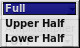
\includegraphics[scale=1.0]{bottom-panel/instrument-edit/PAD/full-upper-lower.jpg}
   \caption{PADsynth Full/Upper/Lower Harmonics}
   \label{fig:padsynth_full_upper_lower}
\end{figure}

   Values: \texttt{Full*, Upper Half, Lower Half}

   \itempar{AmpMultiplier}{padsynth!amp mult}
   Amplitude Multiplier.
   Apply a secondary modulation on top of the profile built thus far; the
   modulating shape can be a bell function (gauss), a sine wave, or just a plateau
   in the center (flat).   These values spread out the frequency components in
   various ways.

\begin{figure}[H]
   \centering
   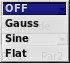
\includegraphics[scale=1.0]{bottom-panel/instrument-edit/PAD/amp-multiplier.jpg}
   \caption{PADsynth Amplitude Multiplier}
   \label{fig:padsynth_amplitude_multiplier}
\end{figure}

   Values: \texttt{OFF*, Gauss, Sine, Flat}

   \itempar{AmpMode}{padsynth!amp mode}
   Amplitude Mode.
   The way this secondary modulation is worked into the profile.

\begin{figure}[H]
   \centering
   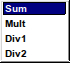
\includegraphics[scale=1.0]{bottom-panel/instrument-edit/PAD/amp-mode.jpg}
   \caption{PADsynth Amplitude Mode}
   \label{fig:padsynth_amplitude_mode}
\end{figure}

   Values: \texttt{Sum*, Mult, Div1, Div2}

   \begin{itemize}
      \item \textbf{Sum}.
         A linear blend between the secondary modulator, and the original
         profile; the fade is controlled by par2
      \item \textbf{Multiply}.
         The profile is filtered by (multiplied with) the modulator; the strength
         of filtering is controlled by par2
      \item \textbf{Div1}.
         The profile is divided by the modulator — where the latter is strong, the
         profile is damped
      \item \textbf{Div2}.
         The modulator is divided by the profile, i.e. the profile is carved out of
         the modulator shape
   \end{itemize}

   \itempar{Par1}{padsynth!harmonic par1}
   Harmonic Parameter 1.
   Squeeze or spread the secondary modulating shape.
   Increasing this parameter narrows the width of the central spectral
   component.

   Values: \texttt{0 to 127}

   \itempar{Par2}{padsynth!harmonic par2}
   Harmonic Parameter 2.
   Controls how the secondary modulation is faded or combined with the harmonic
   profile.  Varying this parameter changes the relative amplitude of the central
   spectral component and the sidebands.

   Values: \texttt{0 to 127}

\subsubsection{PADsynth / Harmonic Structure / Harmonic}
\label{subsubsec:padsynth_harmonic_structure_harmonic}

   \begin{enumber}
      \item \textbf{Profile of One Harmonic}
      \item \textbf{Harmonic Content Window}
      \item \textbf{base}
      \item \textbf{smp/oct}
      \item \textbf{no.oct}
      \item \textbf{Sample Size}
      \item \textbf{Crossfade}
      \item \textbf{Retrigger} (section)
      \item \textbf{Resonance} (section)
      \item \textbf{Change} (section)
   \end{enumber}

   \setcounter{ItemCounter}{0}      % Reset the ItemCounter for this list.

   \itempar{Profile}{padsynth!harmonic profile}
   Profile of One Harmonic (Frequency Distribution).
   Indicates which part of the profile to use: Full (the default), or only the
   upper half, or only the lower half.

   \itempar{Harmonic Content Window}{padsynth!harmonic content}
   Harmonic Content Window.

   \itempar{base}{padsynth!harmonic base}
   The note value for the lowest wavetable generated.

\begin{figure}[H]
   \centering
   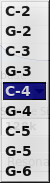
\includegraphics[scale=1.0]{bottom-panel/instrument-edit/PAD/base.jpg}
   \caption{Harmonic Base Dropdown}
   \label{fig:padsynth_harmonic_base_dropdown}
\end{figure}

   Values: \texttt{C-2, G-2, C-3, G-3, C-4*, G-4, C-5, G-5, G-6}

   \itempar{smp/oct}{padsynth!harmonic samples per oct}
   Harmonic Samples Per Octave.
   The number of wavetables generated within each octave.

\begin{figure}[H]
   \centering
   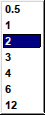
\includegraphics[scale=1.0]{bottom-panel/instrument-edit/PAD/smp-per-octave.jpg}
   \caption{Harmonic Samples Per Octave}
   \label{fig:padsynth_harmonic_samples_per_octave}
\end{figure}

   \itempar{no.oct}{padsynth!harmonic no. of octaves}
   Number of Octaves of Harmonic.
   The number of octaves to cover with dedicated wavetables.

\begin{figure}[H]
   \centering
   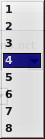
\includegraphics[scale=1.0]{bottom-panel/instrument-edit/PAD/number-of-octaves.jpg}
   \caption{Harmonic Number of Octaves}
   \label{fig:padsynth_harmonic_number_of_octaves}
\end{figure}

   Values: \texttt{1, 2, 3, 4*, 5, 6, 7, 8}

   \itempar{Sample Size}{padsynth!harmonic sample size}
   Harmonic Sample Size.
   Size of the generated wavetable(s). A large wavetable captures more fine
   details of the harmonic profile and gives more time until the patterns repeat,
   but it costs more time to build and it takes up more memory.

\begin{figure}[H]
   \centering
   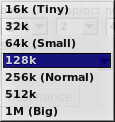
\includegraphics[scale=1.0]{bottom-panel/instrument-edit/PAD/sample-size.jpg}
   \caption{Harmonic Sample Size Dropdown}
   \label{fig:padsynth_harmonic_sample_size_dropdown}
\end{figure}

   \begin{itemize}
      \item \textbf{128k}
         The default value provides 2.6sec of sound at 48kHz sampling rate and
         requires 1/2 MiB.
      \item \textbf{1M (big)}
         The largest possible wavetable holds 21sec of sound until repetition, and
         requires 4 MiB of RAM per table.

   \end{itemize}

   Values: \texttt{16k (Tiny), 32k, 64k (Small), 128k*, 256k (Normal), 512k, 1M
   (Big)}

   \itempar{Crossfade}{padsynth!crossfade}
   Wavetable Fade Time.
   The time it takes to fade from the old wavetable to the new one (for Background
   and Auto-Apply modes).

   Values: \texttt{off, 1mS,200mS*, 20S}

\subsubsection{PADsynth / Harmonic Structure / Bandwidth and Position}
\label{subsubsec:padsynth_harmonic_structure_bw_and_pos}

   \begin{enumber}
      \item \textbf{BandWidth}
      \item \textbf{cents}
      \item \textbf{Bandwidth Scale}
      \item \textbf{Spectrum Mode}
      \item \textbf{OvertonesPosition}
      \item \textbf{Par1}
      \item \textbf{Par2}
      \item \textbf{ForceH}
      \item \textbf{Harmonics Plot}
   \end{enumber}

   \setcounter{ItemCounter}{0}      % Reset the ItemCounter for this list.

   \itempar{AutoScale}{padsynth!autoscale}
   AutoScale.
   Automatically stretches or squeezes the resulting profile, so that all the
   various profile shapes generate a similar blurring effect.
   What is taken as
   \textsl{nominal bandwith} is indicated in the profile display by the vertical
   bars and the dark background.
   If AutoScale is disabled, this nominal bandwidth is fixed
   and thus reshaping the profile also increases or decreases the actual spread.

   \itempar{BandWidth}{padsynth!bandwidth}
   Harmonics Bandwidth.
   This is the most important control, and defines the effective Bandwidth of the
   harmonic profile in cents. By increasing this value, the sound transitions
   gradually from the precise waveform to a sonic cloud.

   Values: \texttt{0 to 127}

   \itempar{cents}{padsynth!bandwidth reading}
   Bandwidth Reading (cents).

   \itempar{Bandwidth Scale}{padsynth!bandwidth scale}
   Bandwidth Scale.
   How the Bandwidth is adjusted with the increasing frequency of each harmonic.

   \begin{itemize}
      \item \textbf{Normal}.
         Bandwith grows with frequency, and thus perceptually the spread is the same
         on each harmonic.
      \item \textbf{EqualHz}.
         Bandwidth is constant, independent of frequency.
         Perceptually this means that the bandwidth on higher harmonics seems to
         diminish.
      \item \textbf{Quarter, Half, 75\%, 150\%, Double}.
         All these setting increase the Bandwith for higher harmonics to various
         degrees.
      \item \textbf{Inv.Half}.
         Here the bandwidth is even reduced for higher harmonics by half an octave
         per octave.

   \end{itemize}

\begin{figure}[H]
   \centering
   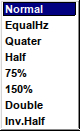
\includegraphics[scale=1.0]{bottom-panel/instrument-edit/PAD/bandwidth-scale.jpg}
   \caption{Harmonics Bandwidth Scale.}
   \label{fig:padsynth_harmonics_bandwidth_scale}
\end{figure}

   Values: \texttt{Normal, EqualHz, Quarter, Half, 75\%, 150\%, Double, Inv.  Half}

   \itempar{Spectrum Mode}{padsynth!spectrum mode}
   Harmonics Spectrum Mode.

   Spectrum Mode defines the way PadSynth generates the spectrum, which is then
   rendered into wavetables.

\begin{figure}[H]
   \centering
   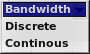
\includegraphics[scale=1.0]{bottom-panel/instrument-edit/PAD/spectrum-mode.jpg}
   \caption{PADsynth Harmonics Spectrum Mode}
   \label{fig:padsynth_harmonics_spectrum mode}
\end{figure}

   \begin{itemize}
      \item \textbf{Bandwidth(default)}.
         Widen each harmonic of the base waveform spectrum with the harmonic
         profile, by an amount controlled through the bandwidth setting and
         bandwidth scale.
      \item \textbf{Discrete}.
         Similar to AddSynth, each harmonic is retained as a sharp line, not using
         bandwidth and profile, yet the overtones position can still be shifted
         and unharmonic.
      \item \textbf{Continuous}.
         Likewise ignoring bandwidth and profile, but this time taken to the other
         extreme; the outline of all harmonics is connected into a common
         distribution and thus rendered into a form of coloured noise.
   \end{itemize}

   Values: \texttt{Bandwidth*, Discrete, Continuous}

   \itempar{OvertonesPosition}{padsynth!overtones}
   Overtones Position.
   Since PadSynth re-renders the partials with high resolution, it is possible to
   shift overtones to non-harmonic positions, to create a wide array of metallic
   and noisy flavours. For Harmonic there is no control, so the other parameters
   are inactive. Similarly Par 2 does nothing for Shift so is disabled for that
   variation.

   \begin{itemize}
      \item \textbf{Harmonic (default)}.
         Overtones are located at exact multiples of the base frequency.
      \item \textbf{Shift}.
         All overtones are spread towards higher pitches.
      \item \textbf{Power}.
         Here the spread is guided by a power function and thus increases
         excessively for higher harmonics;
         Par2 defines the exponent (i.e. the acceleration).
      \item \textbf{ShiftU / ShiftL}.
         Par2 defines a threshold, harmonics above are spread or condensed.
      \item \textbf{PowerU}.
         Par1 defines a turning point, par2 the strength of the effect;
         harmonics are condensed around the turning point by a power function.
      \item \textbf{PowerL}.
         Par1 controls a linear blend between the harmonic positions and positions
         shifed by a power function;
         harmonics are here spread away from a fixed turning point at the 10-th
         overtone.
      \item \textbf{Sine}.
         Harmonics are alternatingly shifted up or down, causing them to cluster;
         par2 defines the frequency and thus the density of these overtone.
   \end{itemize}

\begin{figure}[H]
   \centering
   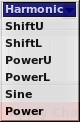
\includegraphics[scale=1.0]{bottom-panel/instrument-edit/PAD/overtones-position.jpg}
   \caption{PADsynth Overtones Position}
   \label{fig:padsynth_overtones_position}
\end{figure}

   Values: \texttt{Harmonic*, ShiftU, ShiftL, PowerU, PowerL, Sine, Power}

   \itempar{Par1}{padsynth!par1}
   PADSynth Bandwidth Parameters 1.
   If the \textbf{Overtones Position} drop-down is set to something other than
   \texttt{Harmonic}, then this knob changes the harmonic lines shown in the
   spectrum view just below this item.
   It is best to play with this setting and observe and hear the changes it
   makes.

   \itempar{Par2}{padsynth!par2}
   PADSynth Bandwidth Parameters 2.
   If the \textbf{Overtones Position} drop-down is set to something other than
   \texttt{Harmonic}, then this knob changes the harmonic lines shown in the
   spectrum view (\textbf{Harmonics Plot}) just below this item.
   It is best to play with this setting and observe and hear the changes it
   makes.

   \itempar{ForceH}{padsynth!forceh}
   PADSynth Bandwidth ForceH.
   If the \textbf{Overtones Position} drop-down is set to something other than
   \texttt{Harmonic}, then this knob changes the harmonic lines shown in the
   spectrum view just below this item.
   It moves the shifted harmonics by a variable amount back towards the nearest
   actual multiple of the fundamental. This allows one to reduce and fine-tune the
   actual amount of \textsl{noisiness}.
   It is best to play with this setting and observe and hear the changes it
   makes.

   \itempar{Harmonics Plot}{padsynth!harmonics plot}
   PADSynth Harmonics Plot.
   Shows the position and amplitude of each of the harmonic lines that the
   settings will generate.

   \textbf{Apply Changes}.
   If any of the above controls for the harmonic profile are altered it will be
   necessary to rebuild the wavetables to hear the effect. Also, be aware that
   with a very big sample size and/or octave range and samples/octave this could
   take many seconds to complete.
   \textsl{Yoshimi} provides several modes to handle these
   PadSynth wavetable builds, which can be configured in the
   \textbf{Global Settings}:

   \begin{itemize}
      \item \textbf{Mute}.
         Build is triggered manually with the Apply button — disable part while
         wavetable is assembled.  This is the legacy mode and should be used if
         the other modes cause audible clicks.
      \item \textbf{Background(default)}.
         Build triggered manually — continue using old wavetables while building
         the new ones in the background; smooth transition with crossfade when
         ready.
      \item \textbf{Auto-Apply}.
         Automatically launch a wavetable build whenever a parameter is changed,
         then crossfade when ready.
   \end{itemize}

\subsubsection{PADsynth / Harmonic Structure / Export}
\label{subsubsec:padsynth_harmonic_structure_export}

\begin{figure}[H]
   \centering
   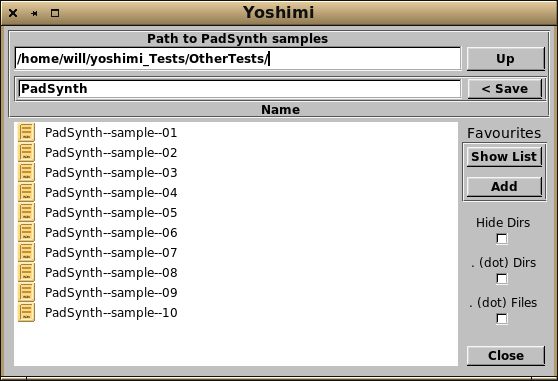
\includegraphics[scale=0.8]{2.0/PadSynthExport.png}
   \caption{Harmonics Structure Export Dialog}
   \label{fig:harmonics_structure_export_dialog}
\end{figure}

   This export dialog is a file dialog similar to other file dialogs
   in \textsl{Yoshimi}.
   It is a filer window for exporting a complete wavetable with the total number
   of samples one has currently set. These don't include any changes in the sound
   produced by controls in the envelopes window.

\subsubsection{PADsynth / Harmonic Structure / Retrigger}
\label{subsubsec:padsynth_harmonic_structure_retrigger}
   This button opens a window for Random regeneration of the wavetable.
   This dialog (new in \textsl{Yoshimi} V2.2.0) has yet to be described.

\begin{figure}[H]
   \centering
   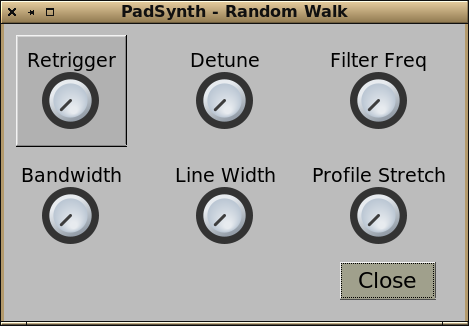
\includegraphics[scale=0.75]{2.2.0/padrandom.png}
   \caption{Random Walk Editor}
   \label{fig:padsynth_random_walk_editor}
\end{figure}

\subsubsection{PADsynth / Harmonic Structure / Resonance}
\label{subsubsec:padsynth_harmonic_structure_resonance}

   This button gives access to an overall Resonance that can be applied to the
   engine.  This dialog, shared in common with the ADDsynth editor, is a stock
   user-interface element described in
   \sectionref{subsec:stock_resonance_settings}.

\subsubsection{PADsynth / Harmonic Structure / Waveform}
\label{subsubsec:padsynth_harmonic_structure_change}

   The \textbf{Waveform} button brings up the
   Harmonic Content editor, which is another complex dialog.
   Like \figureref{fig:addsynth_oscillator_editor},
   it allows one to create an essentially unlimited number of oscillators.
   It is a highly detailed waveshape editor, which is identical to the one
   available in AddSynth — with the exception of the phase control on individual
   partials; PadSynth ignores these and always picks completely random phases,
   whenever building a new wavetable. Note also that one can copy and paste the
   entire settings of this waveform editor between AddSynth and PadSynth; one may
   create a clear and pronounced sound with AddSynth and then take it into
   PadSynth to soften, spread and blur it, while retaining its character.

\begin{figure}[H]
   \centering
   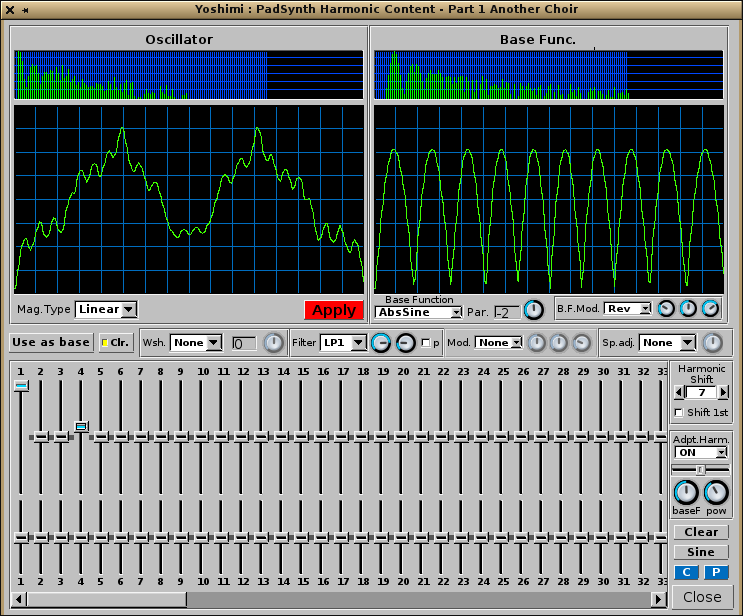
\includegraphics[scale=0.75]{2.0/PadOscillator.png}
   \caption{Harmonic Content Editor}
   \label{fig:padsynth_harmonic_content_editor}
\end{figure}

   This dialog is complex enough that it makes sense to break it down into
   sub-sections.

   \begin{enumber}
      \item \textbf{Oscillator} (section)
      \item \textbf{Base Function} (section)
      \item \textbf{Middle} (section)
      \item \textbf{Harmonic} (section)
   \end{enumber}

\paragraph{PADsynth / Harmonic Structure / Change / Oscillator}
\label{paragraph:padsynth_harmonic_structure_change_oscillator}

   \begin{enumber}
      \item \textbf{Oscillator Spectrum Graph}
      \item \textbf{Oscillator Waveform Graph}
      \item \textbf{Mag.Type}
      \item \textbf{Apply}
   \end{enumber}

   \setcounter{ItemCounter}{0}      % Reset the ItemCounter for this list.

   \itempar{Oscillator Spectrum Graph}{padsynth!oscillator graph}
   Oscillator Spectrum Graph.
   This graph shows the spectrum of the oscillator as a series of vertical
   lines, a kind of frequency histogram.

   \itempar{Oscillator Waveform Graph}{padsynth!waveform graph}
   Oscillator Waveform Graph.
   This graph shows the temporal waveform  of the oscillator.

   \itempar{Mag.Type}{padsynth!mag type}
   Oscillator Magnitude Type.
   Sets how the magnitudes from the user interface behave.  See the values
   below.

\begin{figure}[H]
   \centering
   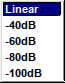
\includegraphics[scale=1.0]{bottom-panel/instrument-edit/PAD/harmonic-content-mag-type.jpg}
   \caption{PADsynth Harmonic Content Mag Type}
   \label{fig:padsynth_harmonic_content_mag_type}
\end{figure}

   Values: \texttt{Linear*, -40dB, -60db, -80dB, -100dB}

   \itempar{Apply}{padsynth!apply button}
   PADsynth Harmonic Content Editor Apply Button.

   \textbf{Note:} This is not present in the ADDsynth oscillator. Instead there are two additional
   controls, as seen with
   \figref{fig:addsynth_wave_controls_extra}.

\begin{figure}[H]
   \centering
   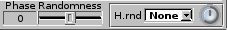
\includegraphics[scale=1.0]{1.6.0/wave_controls_extra.png}
   \caption{ADDsynth Oscillator Extras}
   \label{fig:addsynth_wave_controls_extra}
\end{figure}
    \textbf{Phase Randomness} changes the relative phase of the overall oscillator and is only really
    noticeable when there is more than one voice.

    \textbf{H. rnd} - Harmonic Randomness is very noticeable and (we think) changes the
    \textsl{amplitude} of the harmonics.

\paragraph{PADsynth / Harmonic Structure / Change / Base Function}
\label{paragraph:padsynth_harmonic_structure_change_base_function}

   \begin{enumber}
      \item \textbf{Base Func. Spectrum Graph}
      \item \textbf{Base Func. Waveform Graph}
      \item \textbf{Base F..}
      \item \textbf{Par. Value}
      \item \textbf{Par. Wheel}
      \item \textbf{B.F.Mod.}
      \item \textbf{Wheel 1}
      \item \textbf{Wheel 2}
      \item \textbf{Wheel 3}
   \end{enumber}

   \setcounter{ItemCounter}{0}      % Reset the ItemCounter for this list.

   \itempar{Base Func. Spectrum Graph}{padsynth!base function spectrum}
   Harmonic Base Function Spectrum Graph.

   \itempar{Base Func. Waveform Graph}{padsynth!base function waveform}
   Harmonic Base Function Waveform Graph.

   \itempar{Base F}{padsynth!base function}
   Harmonic Base Function.
   Sets what function to use as the harmonics base function.
   One can use any base function as harmonics.

\begin{figure}[H]
   \centering
   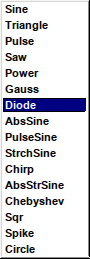
\includegraphics[scale=1.0]{bottom-panel/instrument-edit/PAD/harmonic-content-base-function.jpg}
   \caption{PADsynth Harmonic Content Base Function}
   \label{fig:padsynth_harmonic_content_base_function}
\end{figure}

   Values: \texttt{Sine*, Triangle, Pulse, Saw, Power, Gauss, Diode, AbsSine,
           PulseSine, StrchSine, Chirp, AbsStrSine, Chebyshev,
           Sqr, Spike, Circle}

   \itempar{Par. Value}{padsynth!par value}
   PADsynth Parameter Value.

   \itempar{Par. Wheel}{padsynth!par wheel}
   PADsynth Parameter Wheel.
   Change the parameter of the base function.

   \itempar{B.F.Mod}{padsynth!bf mod}
   PADSynth Base Frequency Mod.
   This item is very similar to the Harmonic Editor Modulation
   (\textbf{Mod.}) setting.

   Values: \texttt{None*, Rev, Sine, Pow}

   \itempar{Wheel 1}{padsynth!wheel 1}
   PADsynth Wheel 1.
   With the \textbf{B.F.Mod.} selection set to something other than
   \texttt{None}, this modifies one (unknown at this time) parameter of the
   modulation selection.

   \itempar{Wheel 2}{padsynth!wheel 2}
   PADsynth Wheel 2.
   With the \textbf{B.F.Mod.} selection set to something other than
   \texttt{None}, this modifies one (unknown at this time) parameter of the
   modulation selection.

   \itempar{Wheel 3}{padsynth!wheel 3}
   PADsynth Wheel 3.
   With the \textbf{B.F.Mod.} selection set to something other than
   \texttt{None}, this modifies one (unknown at this time) parameter of the
   modulation selection.

\paragraph{PADsynth / Harmonic Structure / Change / Middle}
\label{paragraph:padsynth_harmonic_structure_change_middle}

   \begin{enumber}
      \item \textbf{Use as base}
      \item \textbf{Clr.}
      \item \textbf{Wsh.}
      \item \textbf{Wsh Value}
      \item \textbf{Wsh Wheel}
      \item \textbf{Filter}
      \item \textbf{Filter Wheel 1}
      \item \textbf{Filter Wheel 2}
      \item \textbf{Filter p}
      \item \textbf{Mod.}
      \item \textbf{Mod. Wheel 1}
      \item \textbf{Mod. Wheel 2}
      \item \textbf{Mod. Wheel 3}
      \item \textbf{Sp.adj.}
      \item \textbf{Sp.adj. Wheel}
   \end{enumber}

   \setcounter{ItemCounter}{0}      % Reset the ItemCounter for this list.

   \itempar{Use as base}{padsynth!harm editor use-as-base}
   Use as Base.
   Convert the oscillator output to a base function. Changing the Base
   function or its parameter will erase the converted base function.

%  We've cured a long-standing anomally, where setting up
%  a complex waveshape, then clicking the \textbf{Use as Base} button
%  do all the necessary conversions, but would leave the base function showing
%  the original.  Now it shows 'User', which is normally hidden and is a
%  non-selectable entry.

   \itempar{Clr}{padsynth!harm editor clr}
   Clear.
   Clear the settings and make the oscillator equal to a base function. If
   this is cleared, one can click the \textbf{Use as base} button to make
   multiple conversions to base functions.

   \itempar{Wsh}{padsynth!harm editor wsh}
   Harmonic Editor Wave-shaping, "W.sh".

   Wave shaping function that applies to the oscillator.
   It has one parameter that fine-tunes the wave-shaping function.

   \itempar{Wsh Value}{padsynth!harm editor wsh value}
   Harmonic Editor Wave-shaping Value.

\begin{figure}[H]
   \centering
   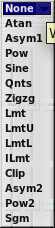
\includegraphics[scale=1.0]{bottom-panel/instrument-edit/PAD/harmonic-content-waveshaping-function.jpg}
   \caption{PADsynth Harmonic Content Editor Wave-Shaping Function}
   \label{fig:padsynth_harmonic_content_editor_waveshaping_function}
\end{figure}

   Values: \texttt{None*, Atan, Asym1, Pow, Sine, Qnts, Zigzg, Lmt,
              LmtU, LmtL, ILmt, Clip, Asym2, Pow2, Sgm}

   The type of wave-shaping distortion has much influence on how the
   overtones are being placed. Sometimes, one gets a "fat" bass, and
   sometimes, high frequencies are added, making the sound "crystal clear".

   \textbf{Atan \& Sigmoid}.
   This is the default setting. It is an easy way to apply loudness to a wave
   without getting undesired high overtones. Thus, it can be used both for
   making instruments that sound like "real" ones, but also for electronic
   music. The transformation turns, roughly said, every amplitude into a
   square amplitude. Thus, sine, power, pulse and triangle turn into a usual
   square wave, while a saw turns into a phased square wave. A chirp wave
   turns into a kind of phase modulated square wave.

   \textbf{Quants} ("Qnts")
   Quantisation adds high overtones early. It can be seen as an unnatural
   effect, which is often used for electronic music.  The transformation is a
   bit similar to building the lower sum of a wave, mathematically said. This
   means that the transformation effect turns an "endless high" sampled
   wave into only a few samples. The more distortion one applies, the fewer
   samples will be used. Indeed, this is equivalent to say that more input
   amplification is used.
%   To see this, here is a small sample of code, where
%   "ws" is the (correctly scaled amount of input amplification, and "n" the
%   number of original samples.

%  WHERE IS THE CODE?

   If one turns on quantisation very high, one might be confused that,
   especially high notes, make no sound. The reason: High frequencies are
   "forgotten" if one samples with only few samples. Also, the sign of an
   amplitude can be forgotten. This behaviour might make some quantisations a
   bit unexpected.

   \textbf{Limiting} ("Lmt*" and "Clip")
   Limiting usually means that for a signal, the amplitude is modified
   because it exceeds its maximum value. Overdrive, as often used for
   guitars, is often achieved by limiting: It happens because an amplifier
   "overdrives" the maximum amplitude it can deliver.

   \textsl{Yoshimi} has two types of limiting. Soft limiting, here as Lmt, means
   that the sound may not exceed a certain value. If the amplitude does so,
   it will simply be reduced to the limiting value. The overtones are
   generated in the lower frequencies first.

   Hard limiting, is also called clipping and abbreviated Clip. This means
   that if the maximum is exceeded, instead of being constant at the limiting
   value, the original signal still has some influence on the output signal.
   Still, it does not exceed the limiting value. For \textsl{Yoshimi}, a signal
   exceeding the limiting value will continue to grow "in the negative". This
   leads to overtones being generated on the full frequency band.

   \itempar{Wsh Wheel}{padsynth!harm editor wsh wheel}
   Harmonic Editor Wave-shaping Wheel.

   \itempar{Filter}{padsynth!harm editor filter}
   Harmonic Editor Filter.
   Sets the type of the harmonic filter.

\begin{figure}[H]
   \centering
   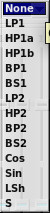
\includegraphics[scale=1.0]{bottom-panel/instrument-edit/PAD/harmonic-content-filter.jpg}
   \caption{PADsynth Harmonic Content Filter}
   \label{fig:}
\end{figure}

   Values: \texttt{None*, LP1, HP1a, HP1b, BP1, BS1, LP2, HP2, BP2,
              BS2, Cos, Sin, LSh, S}

   \itempar{Filter Wheel 1}{padsynth!harm editor filter wheel}
   Harmonic Editor Filter, Wheel 1.
   The knob on the left sets one filter parameter, which is either the cutoff
   frequency, or, if the filter is a bandpass filter, the lower corner
   frequency.
   It is best to play with this knob with various kinds of filters selected
   from the filter drop-down list.

   \itempar{Filter Wheel 2}{padsynth!harm editor filter wheel}
   Harmonic Editor Filter, Wheel 2.
   The knob on the right sets, if the filter is a bandpass filter, the upper
   corner frequency.
   It is best to play with this knob with various kinds of filters selected
   from the filter drop-down list.

   \itempar{Filter p}{padsynth!harm editor filter p}
   Harmonic Editor Filter, p.
   If set, the filter is applied before waveshaping.

   \itempar{Mod}{padsynth!harm editor mod}
   Harmonic Editor Modulation.

\begin{figure}[H]
   \centering
   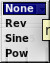
\includegraphics[scale=1.0]{bottom-panel/instrument-edit/PAD/harmonic-content-modulation.jpg}
   \caption{PADsynth Harmonic Content Editor Modulation}
   \label{fig:padsynth_harmonic_content_editor_modulation}
\end{figure}

   Values: \texttt{None*, Rev, Sine, Pow}

   \itempar{Mod. Wheel 1}{padsynth!harm editor mod wheel}
   Harmonic Editor Modulation Wheel 1.
   With the \textbf{Mod.} selection set to something other than
   \texttt{None}, this modifies one (unknown at this time) parameter of the
   modulation selection.

   \itempar{Mod. Wheel 2}{padsynth!harm editor mod wheel}
   Harmonic Editor Modulation Wheel 2.
   With the \textbf{Mod.} selection set to something other than
   \texttt{None}, this modifies one (unknown at this time) parameter of the
   modulation selection.

   \itempar{Mod. Wheel 3}{padsynth!harm editor mod wheel}
   Harmonic Editor Modulation Wheel 3.
   With the \textbf{Mod.} selection set to something other than
   \texttt{None}, this modifies one (unknown at this time) parameter of the
   modulation selection.

   \itempar{Sp.adj}{padsynth!harm editor spadj}
   Harmonic Editor Spectrum Adjust.
   Adjust the spectrum of the waveform.

   RMS normalize. Enables the RMS normalization method (recommended); this
   keeps the same loudness regardless the harmonic content.

   Below are the harmonics and their phases. One can use them to add to
   oscillator harmonics that has the waveform of the base function.
   Increasing the number of harmonics has virtually no effect on CPU usage.
   Right click to set a harmonic/phase to the default value.

\begin{figure}[H]
   \centering
   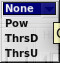
\includegraphics[scale=1.0]{bottom-panel/instrument-edit/PAD/harmonic-content-osc-spectrum-adjust.jpg}
   \caption{PADsynth Harmonic Content Editor Spectrum Adjust}
   \label{fig:padsynth_harmonic_content_editor_spectrum_adjust}
\end{figure}

   Values: \texttt{None*, Pow, ThrsD, ThrsU}

   \itempar{Sp.adj. Wheel}{padsynth!harm editor spadj wheel}
   Harmonic Editor Spectrum Adjust Wheel.

\paragraph{PADsynth / Harmonic Structure / Change / Harmonic}
\label{paragraph:padsynth_harmonic_structure_change_harmonic}

   \begin{enumber}
      \item \textbf{Harmonics Amplitude}
      \item \textbf{Harmonics Bandwidth}
      \item \textbf{Harmonics Scrollbar}
      \item \textbf{Harmonic Shift}
      \item \textbf{Harmonic Shift R}
      \item \textbf{Harmonic Shift preH}
      \item \textbf{Adpt.Harm.}
      \item \textbf{Adpt.Harm. Slider}
      \item \textbf{Adpt.Harm. baseF}
      \item \textbf{Adpt.Harm. pow}
      \item \textbf{Clear}
      \item \textbf{Sine}
      \item \textbf{C}
      \item \textbf{P}
      \item \textbf{Close}
   \end{enumber}

   \itempar{Harmonics Amplitude}{padsynth!harmonics amplitude}
   Harmonics Amplitude.
   Provides 128 sliders for the amplitude of harmonics.

   Values: \texttt{-100\%, 0*, 100\%}

   \itempar{Harmonics Bandwidth}{padsynth!harmonics bandwidth}
   Harmonics Bandwidth.
   Provides 128 sliders for the bandwidth of harmonics.

   Values: \texttt{-88.6, 0*, 90} (degrees)

   \itempar{Harmonics Scrollbar}{padsynth!harmonics scrollbar}
   Harmonics Scrollbar.

   \itempar{Harmonic Shift}{padsynth!harmonics shift}
   Harmonics Shift.

   \itempar{Harmonic Shift R}{padsynth!harmonics shift r}
   Harmonics Shift Reset.
   Pressing this button resets the \textbf{Harmonic Shift} value to zero
   (0).

   \itempar{Harmonic Shift preH}{padsynth!harmonics shift preh}
   Harmonics Shift preH.
   If set, applies the harmonic shift before the filtering and waveshaping.

   \itempar{Adpt.Harm}{padsynth!harmonics}
   Adaptive Harmonics.
   Changes the type of the adaptive harmonics.
   (The tooltip spells "adaptive" wrong.)

\begin{figure}[H]
   \centering
   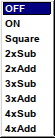
\includegraphics[scale=1.0]{bottom-panel/instrument-edit/PAD/harmonic-content-adaptive-harmonic-type.jpg}
   \caption{PADsynth Adaptive Harmonic Type}
   \label{fig:padsynth_adaptive_harmonic_type}
\end{figure}

   Values: \texttt{OFF*, ON, Square, 2xSub, 2xAdd, 3xSub, 3xAdd, 4xSub, 4xAdd}

   \itempar{Adpt.Harm. Slider}{padsynth!harmonics slider}
   Adaptive Harmonics Slider.
   If something other than \texttt{OFF} or \texttt{ON} is selected,
   then this slider changes the waveform appearance.
   Even more informative is the change in the spectrum that is shown.
   This setting is something to play with while listening to the
   waveform.

   \itempar{Adpt.Harm. baseF}{padsynth!harmonics basef}
   Adaptive Harmonics Base Frequency.
   If something other that \texttt{OFF} is selected,
   then this knob changes the waveform appearance.
   Even more informative is the change in the spectrum that is shown.
   This setting is also something to play with while listening to the
   waveform.

   \itempar{Adpt.Harm. pow}{padsynth!harmonics pow}
   Adaptive Harmonics Power.
   If something other that \texttt{OFF} is selected,
   then this knob changes the waveform appearance.
   Even more informative is the change in the spectrum that is shown.
   Again, this setting is something to play with while listening to the
   waveform.

   \itempar{Clear}{padsynth!harmonics clear}
   Harmonics Clear.
   Clears the harmonics settings.

   \itempar{Sine}{padsynth!harmonics sine}
   Harmonics Sine.
   The user is prompted to "Convert to sine?"
   This seems simply to reset the base function to a sine wave.

   \itempar{C}{padsynth!harmonics copy}
   Harmonics Copy.

   \itempar{P}{padsynth!harmonics paste}
   Harmonics Paste.

   \itempar{Close}{padsynth!harmonics close}
   Harmonics Close.

\subsection{PADsynth / Envelopes and LFOs}
\label{subsec:padsynth_envelopes_lfos}

   This dialog is reached by click on the \textbf{Envelopes LFOs}
   tab of the PADsynth parameters dialog.  This tab is next to the
   \textbf{Harmonic Structure} tab.

   This view consists of nothing but stock user-interface elements that are
   described elsewhere in this manual.
   The Volume and Panning values and ranges are identical to the ADDsynth
   global ones.
   None of these affect the wavetable itself, so there is no need for the apply
   button here.

\begin{figure}[H]
   \centering
%  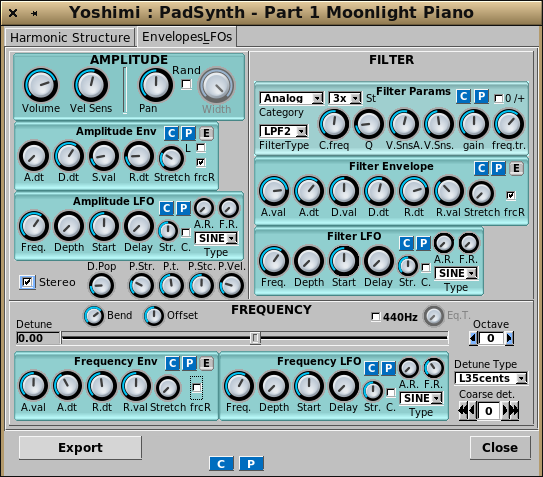
\includegraphics[scale=1.0]{2.0/PadSynthEnvelopes.png}
   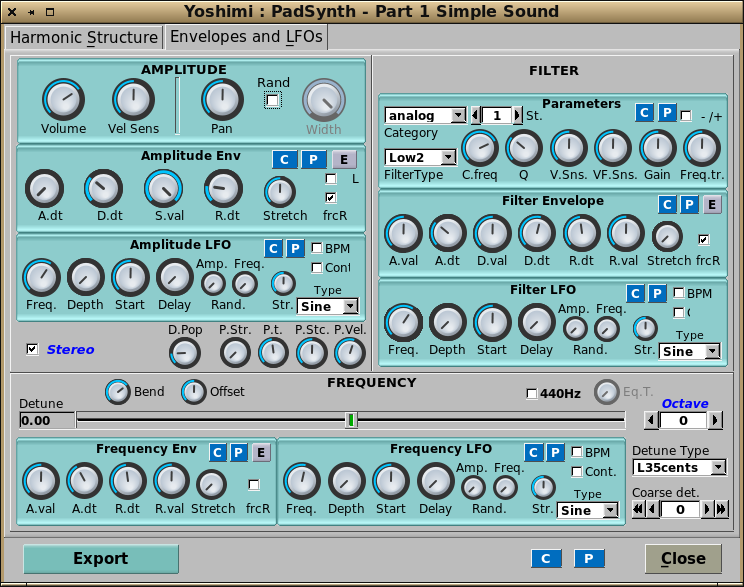
\includegraphics[scale=0.65]{2.1.2/padenvelope.png}
   \caption{PADSynth Parameters, Envelopes and LFOs}
   \label{fig:padsynth_parameters_envelopes_and_lfos}
\end{figure}

   \begin{enumber}
      \item \textbf{AMPLITUDE}
      \item \textbf{FILTER} (section)
      \item \textbf{FREQUENCY} (section)
      \item \textbf{Export}
      \item \textbf{C}
      \item \textbf{P}
      \item \textbf{Close}
   \end{enumber}

   Note the "Filter Envelope" section in the figure.  This is a free-edit
   version of the envelope.  The non-free-edit view can be seen in
   \figureref{fig:filter_env}, which describes this user-interface item in more
   detail.

   \itempar{AMPLITUDE}{padsynth!amplitude section}
   See \sectionref{subsec:addsynth_amplitude}.
   This stock dialog section provides volume, velocity sensing, panning, an
   amplitude envelope sub-panel, and an amplitude LFO sub-panel.

   \itempar{FILTER}{padsynth!amplitude section}
   See \sectionref{subsec:addsynth_filter}.

   \itempar{FREQUENCY}{padsynth!amplitude section}
   See \sectionref{subsec:addsynth_frequency}.

   \itempar{Export}{padsynth!export}
   Very similar to
   \figureref{fig:harmonics_structure_export_dialog}.

   \itempar{C}{padsynth!copy}
   The stock copy dialog.

   \itempar{P}{padsynth!paste}
   The stock paste dialog.

   \itempar{Close}{padsynth!close}
   Close.

%-------------------------------------------------------------------------------
% vim: ts=3 sw=3 et ft=tex
%-------------------------------------------------------------------------------
